\documentclass[]{book}
\usepackage{lmodern}
\usepackage{amssymb,amsmath}
\usepackage{ifxetex,ifluatex}
\usepackage{fixltx2e} % provides \textsubscript
\ifnum 0\ifxetex 1\fi\ifluatex 1\fi=0 % if pdftex
  \usepackage[T1]{fontenc}
  \usepackage[utf8]{inputenc}
\else % if luatex or xelatex
  \ifxetex
    \usepackage{mathspec}
  \else
    \usepackage{fontspec}
  \fi
  \defaultfontfeatures{Ligatures=TeX,Scale=MatchLowercase}
\fi
% use upquote if available, for straight quotes in verbatim environments
\IfFileExists{upquote.sty}{\usepackage{upquote}}{}
% use microtype if available
\IfFileExists{microtype.sty}{%
\usepackage{microtype}
\UseMicrotypeSet[protrusion]{basicmath} % disable protrusion for tt fonts
}{}
\usepackage[margin=1in]{geometry}
\usepackage{hyperref}
\hypersetup{unicode=true,
            pdftitle={respR -- R Package Documentation},
            pdfauthor={Januar Harianto and Nicholas Carey},
            pdfborder={0 0 0},
            breaklinks=true}
\urlstyle{same}  % don't use monospace font for urls
\usepackage{natbib}
\bibliographystyle{apalike}
\usepackage{color}
\usepackage{fancyvrb}
\newcommand{\VerbBar}{|}
\newcommand{\VERB}{\Verb[commandchars=\\\{\}]}
\DefineVerbatimEnvironment{Highlighting}{Verbatim}{commandchars=\\\{\}}
% Add ',fontsize=\small' for more characters per line
\usepackage{framed}
\definecolor{shadecolor}{RGB}{248,248,248}
\newenvironment{Shaded}{\begin{snugshade}}{\end{snugshade}}
\newcommand{\KeywordTok}[1]{\textcolor[rgb]{0.13,0.29,0.53}{\textbf{#1}}}
\newcommand{\DataTypeTok}[1]{\textcolor[rgb]{0.13,0.29,0.53}{#1}}
\newcommand{\DecValTok}[1]{\textcolor[rgb]{0.00,0.00,0.81}{#1}}
\newcommand{\BaseNTok}[1]{\textcolor[rgb]{0.00,0.00,0.81}{#1}}
\newcommand{\FloatTok}[1]{\textcolor[rgb]{0.00,0.00,0.81}{#1}}
\newcommand{\ConstantTok}[1]{\textcolor[rgb]{0.00,0.00,0.00}{#1}}
\newcommand{\CharTok}[1]{\textcolor[rgb]{0.31,0.60,0.02}{#1}}
\newcommand{\SpecialCharTok}[1]{\textcolor[rgb]{0.00,0.00,0.00}{#1}}
\newcommand{\StringTok}[1]{\textcolor[rgb]{0.31,0.60,0.02}{#1}}
\newcommand{\VerbatimStringTok}[1]{\textcolor[rgb]{0.31,0.60,0.02}{#1}}
\newcommand{\SpecialStringTok}[1]{\textcolor[rgb]{0.31,0.60,0.02}{#1}}
\newcommand{\ImportTok}[1]{#1}
\newcommand{\CommentTok}[1]{\textcolor[rgb]{0.56,0.35,0.01}{\textit{#1}}}
\newcommand{\DocumentationTok}[1]{\textcolor[rgb]{0.56,0.35,0.01}{\textbf{\textit{#1}}}}
\newcommand{\AnnotationTok}[1]{\textcolor[rgb]{0.56,0.35,0.01}{\textbf{\textit{#1}}}}
\newcommand{\CommentVarTok}[1]{\textcolor[rgb]{0.56,0.35,0.01}{\textbf{\textit{#1}}}}
\newcommand{\OtherTok}[1]{\textcolor[rgb]{0.56,0.35,0.01}{#1}}
\newcommand{\FunctionTok}[1]{\textcolor[rgb]{0.00,0.00,0.00}{#1}}
\newcommand{\VariableTok}[1]{\textcolor[rgb]{0.00,0.00,0.00}{#1}}
\newcommand{\ControlFlowTok}[1]{\textcolor[rgb]{0.13,0.29,0.53}{\textbf{#1}}}
\newcommand{\OperatorTok}[1]{\textcolor[rgb]{0.81,0.36,0.00}{\textbf{#1}}}
\newcommand{\BuiltInTok}[1]{#1}
\newcommand{\ExtensionTok}[1]{#1}
\newcommand{\PreprocessorTok}[1]{\textcolor[rgb]{0.56,0.35,0.01}{\textit{#1}}}
\newcommand{\AttributeTok}[1]{\textcolor[rgb]{0.77,0.63,0.00}{#1}}
\newcommand{\RegionMarkerTok}[1]{#1}
\newcommand{\InformationTok}[1]{\textcolor[rgb]{0.56,0.35,0.01}{\textbf{\textit{#1}}}}
\newcommand{\WarningTok}[1]{\textcolor[rgb]{0.56,0.35,0.01}{\textbf{\textit{#1}}}}
\newcommand{\AlertTok}[1]{\textcolor[rgb]{0.94,0.16,0.16}{#1}}
\newcommand{\ErrorTok}[1]{\textcolor[rgb]{0.64,0.00,0.00}{\textbf{#1}}}
\newcommand{\NormalTok}[1]{#1}
\usepackage{longtable,booktabs}
\usepackage{graphicx,grffile}
\makeatletter
\def\maxwidth{\ifdim\Gin@nat@width>\linewidth\linewidth\else\Gin@nat@width\fi}
\def\maxheight{\ifdim\Gin@nat@height>\textheight\textheight\else\Gin@nat@height\fi}
\makeatother
% Scale images if necessary, so that they will not overflow the page
% margins by default, and it is still possible to overwrite the defaults
% using explicit options in \includegraphics[width, height, ...]{}
\setkeys{Gin}{width=\maxwidth,height=\maxheight,keepaspectratio}
\IfFileExists{parskip.sty}{%
\usepackage{parskip}
}{% else
\setlength{\parindent}{0pt}
\setlength{\parskip}{6pt plus 2pt minus 1pt}
}
\setlength{\emergencystretch}{3em}  % prevent overfull lines
\providecommand{\tightlist}{%
  \setlength{\itemsep}{0pt}\setlength{\parskip}{0pt}}
\setcounter{secnumdepth}{5}
% Redefines (sub)paragraphs to behave more like sections
\ifx\paragraph\undefined\else
\let\oldparagraph\paragraph
\renewcommand{\paragraph}[1]{\oldparagraph{#1}\mbox{}}
\fi
\ifx\subparagraph\undefined\else
\let\oldsubparagraph\subparagraph
\renewcommand{\subparagraph}[1]{\oldsubparagraph{#1}\mbox{}}
\fi

%%% Use protect on footnotes to avoid problems with footnotes in titles
\let\rmarkdownfootnote\footnote%
\def\footnote{\protect\rmarkdownfootnote}

%%% Change title format to be more compact
\usepackage{titling}

% Create subtitle command for use in maketitle
\newcommand{\subtitle}[1]{
  \posttitle{
    \begin{center}\large#1\end{center}
    }
}

\setlength{\droptitle}{-2em}

  \title{respR -- R Package Documentation}
    \pretitle{\vspace{\droptitle}\centering\huge}
  \posttitle{\par}
    \author{\textbf{Januar Harianto} and \textbf{Nicholas Carey}}
    \preauthor{\centering\large\emph}
  \postauthor{\par}
    \date{}
    \predate{}\postdate{}
  
\usepackage{booktabs}

\begin{document}
\maketitle

{
\setcounter{tocdepth}{1}
\tableofcontents
}
\chapter{Introduction}\label{introduction}

The R package \texttt{respR} provides a structural, reproducible
workflow for the processing and analysis of respirometry data. Although
the focus of the package is on aquatic respirometry, Functions in
\texttt{respR} are largely unitless and can be used for the analysis of
linear relationships in any time-series data. All analytical methods
used in the package have been peer-reviewed and rigorously tested.

Use \texttt{respR} to:

\begin{itemize}
\tightlist
\item
  automatically \textbf{import} raw data from various oxygen sensing
  equipment;
\item
  rapidly \textbf{test} data for issues before analysis;
\item
  \textbf{explore} and visualise timeseries data;
\item
  perform \textbf{regression} statistics on linear segments of data
  manually or automatically;
\item
  \textbf{convert} units of oxygen consumption; and
\item
  \textbf{export} results quickly for reporting.
\end{itemize}

The goal of this guide is to walk you through the \texttt{respR} package
to import, analyse and convert your data. To begin, you will need to
\protect\hyperlink{installation}{install the package}.

\hypertarget{installation}{\chapter{Installation}\label{installation}}

Use the \texttt{devtools} package to install a stable version of
\texttt{respR}:

\begin{Shaded}
\begin{Highlighting}[]
\CommentTok{# install devtools}
\KeywordTok{install.packages}\NormalTok{(}\StringTok{"devtools"}\NormalTok{)}
\CommentTok{# use devtools to install respR from GitHub}
\NormalTok{devtools}\OperatorTok{::}\KeywordTok{install_github}\NormalTok{(}\StringTok{"januarharianto/respR"}\NormalTok{)}
\end{Highlighting}
\end{Shaded}

The developmental version is mostly stable, and contains some features
that are undergoing peer-review. You may install this version using the
code:

\begin{Shaded}
\begin{Highlighting}[]
\CommentTok{# install dev version}
\NormalTok{devtools}\OperatorTok{::}\KeywordTok{install_github}\NormalTok{(}\StringTok{"januarharianto/respR"}\NormalTok{, }\DataTypeTok{ref =} \StringTok{"develop"}\NormalTok{)}
\end{Highlighting}
\end{Shaded}

Once \texttt{respR} has been installed, load the package into your
workspace:

\begin{Shaded}
\begin{Highlighting}[]
\KeywordTok{library}\NormalTok{(respR)}
\end{Highlighting}
\end{Shaded}

Check out our {[}Quick start{]}{[}quick start{]} guide if you are using
\texttt{respR} for the first time. The
\protect\hyperlink{getting-started}{Getting started} vignette provides a
detailed introduction to respirometry and information about other
vignettes in this document.

\part*{VIGNETTES}\label{part-vignettes}
\addcontentsline{toc}{part}{VIGNETTES}

\hypertarget{getting-started}{\chapter{Getting
started}\label{getting-started}}

\section{Aquatic Respirometry}\label{aquatic-respirometry}

There are four broad methodological approaches in aquatic respirometry:
\emph{closed-chamber}, \emph{intermittent-flow}, \emph{flow-through} and
\emph{open-tank}.

In \textbf{closed-chamber} respirometry, \(O_2\) decrease is measured
within a hermetically sealed chamber of known volume, sometimes set
within a closed loop to allow mixing of the environment within the
chamber. Oxygen recordings may be continuous through use of an oxygen
probe, periodic through withdrawing water or gas samples at set
intervals, or a two-point measurement consisting of the initial and
final concentrations. Metabolic rates are estimated from the \(O_2\)
timeseries by assuming a linear relationship between variables, and
estimates of metabolic rate are straightforward in constant volume
respirometry using the equation: \[VO_2 = \dot O_2V\] where \(\dot O_2\)
is the slope of the regression that describes the rate of change in
\(O_2\) concentration over time, or in the case of a two-point
measurement, the difference in \(O_2\) concentration divided by time
elapsed, and \(V\) is the volume of fluid in the container (Lighton
2008).

In \textbf{intermittent-flow} respirometry, \(O_2\) concentration is
measured as described above, but periodically the chamber is flushed
with new water or air, returning it to initial conditions, resealed, and
the experiment repeated (Svendsen et al. 2016). This technique is
essentially the same as closed respirometry, but with the ability to
conduct replicates easily. Depending on the metabolic rate metric being
investigated, final respiration rate can be calculated as the mean of
the measures (e.g.~Carey et al. 2016), or the lowest or highest rates
recorded in any trial (e.g.~Stoffels 2015).

\textbf{Flow-through} respirometry involves a closed chamber, but with a
regulated flow of air or water through it at a precisely determined
rate. After equilibrium has been achieved, the oxygen concentration
differential between the incurrent and excurrent channels, along with
the flow rate, allows calculation of the oxygen extracted from the flow
volume per unit time: \[\dot{V}O_2 = (C_iO_2 - C_eO_2)FR\] where
\(\dot{V}O_2\) is the rate of \(O_2\) consumption over time, \(C_iO_2\)
and \(C_eO_2\) are the incurrent and excurrent \(O_2\) concentrations,
and \(FR\) is the flow rate through the system (Lighton 2008).

A final method is \textbf{open-tank} respirometry, in which a tank or
semi-enclosed area open to the atmosphere is used, but the input or
mixing rate of oxygen from the surroundings has been quantified or found
to be negligible relative to oxygen consumption of the specimens
(Leclercq et al. 1999). It is seldom used, but for some applications it
is a sufficient and practical methodology (Gamble et al. 2014). The
common equation used for open respirometry is:
\[\dot{V}O_2 = \dot O_2V + \phi_d\] where \(\dot O_2V\) is the slope of
the regression that relates \(O_2\) concentration to time, \(V\) is the
volume of the arena and \(\phi_d\) is the oxygen flux as determined by
Fick's Law (Leclercq et al. 1999).

\section{\texorpdfstring{The \texttt{respR} R
package}{The respR R package}}\label{the-respr-r-package}

\texttt{respR} is a package designed to process the data from all of
these types of respirometry experiment. It is designed primarily for
aquatic respirometry, although because many of the main functions are
unitless it is adaptable for use with gaseous respirometry, and indeed
analysis of other data where a parameter may change over time.

When working with respirometry data, you will often need to:

\begin{enumerate}
\def\labelenumi{\arabic{enumi}.}
\tightlist
\item
  Ensure that the data, or at least a \textbf{subset} of the data, is
  representative of the research question of interest.
\item
  Perform an initial analysis of the data to \textbf{estimate} the rate
  of change in oxygen concentration or amount.
\item
  Depending on the experimental setup, \textbf{correct} for background
  usage of oxygen by micro-organisms, or correct for oxygen flux from
  the air.
\item
  \textbf{Convert} the resulting usage rate to the volumetric and
  mass-specific rates in the appropriate units.
\end{enumerate}

The \texttt{respR} package allows determination of common respirometry
metrics and contains several functions to make this process
straightforward.

\begin{itemize}
\tightlist
\item
  It provides visual feedback and diagnostic plots to help you explore,
  subset and analyse your data.
\item
  It uses computational techniques such as \emph{rolling regressions}
  and \emph{kernel density estimates} to determine \textbf{maximum},
  \textbf{minimum} or \textbf{most linear} rates within time-series
  data.
\item
  The package takes an object-oriented approach, with all functions
  outputting objects which can be read by subsequent functions.
\item
  By separating the workflow into a series of connected functions, you
  can ``mix and match'' functions to help you achieve your result.
\item
  Output objects can also be saved or exported, and contain all raw
  data, parameters used in calculations, and results, allowing for a
  fully documented and reproducibile analysis of respirometry data.
\end{itemize}

\section{Example Data}\label{example-data}

We have provided example data that can be used immediately once
\texttt{respR} is loaded (\texttt{urchins.rd()},
\texttt{intermittent.rd()}, \texttt{zeb\_intermittent.rd()},
\texttt{sardine.rd()}, \texttt{squid.rd()}, \texttt{flowthrough.rd()}).

\begin{Shaded}
\begin{Highlighting}[]
\KeywordTok{data}\NormalTok{(}\DataTypeTok{package =} \StringTok{"respR"}\NormalTok{)}
\end{Highlighting}
\end{Shaded}

These data were obtained from actual experiments and more information
can be obtained by invoking the \texttt{?} command in the R console, for
instance, \texttt{?urchins.rd}.

\section{Vignettes and documentation}\label{vignettes-and-documentation}

We have prepared several vignettes describing typical analysis workflows
and how \texttt{respR} works:

\begin{enumerate}
\def\labelenumi{\arabic{enumi}.}
\item
  \textbf{\href{https://januarharianto.github.io/respR/articles/importing.html}{Importing
  your data}}\\
  \texttt{respR} has functions to make it easy to bring in and prepare
  your data, even from the raw data files output by various respirometry
  systems.
\item
  \textbf{\href{https://januarharianto.github.io/respR/articles/closed.html}{Closed-chamber
  respirometry}}\\
  This is a good place to start to understand the full functionality of
  \texttt{respR}. It describes an entire workflow to process and analyse
  a closed-chamber respirometry dataset.
\item
  \textbf{\href{https://januarharianto.github.io/respR/articles/auto_rate.html}{auto\_rate:
  Automatic detection of metabolic rates}}\\
  Here we introduce the function \texttt{auto\_rate()} for the automatic
  detection and estimation of \textbf{maximum}, \textbf{minimum} and
  \textbf{most linear} rates.
\item
  \textbf{\href{https://januarharianto.github.io/respR/articles/performance.html}{Performance
  of auto\_rate in detecting linear regions}}\\
  We use simulated data to test the accuracy of \texttt{auto\_rate()},
  and discuss the function's performance with focus on linear data
  detection.
\item
  \textbf{\href{https://januarharianto.github.io/respR/articles/auto_rate_comp.html}{Comparative
  performance of auto\_rate and LoLinR}}\\
  We make comparisons to another R package, \texttt{LoLinR}, using data
  from their package and simulated data.
\item
  \textbf{\href{https://januarharianto.github.io/respR/articles/intermittent.html}{Intermittent-flow
  respirometry: Simple example}}\\
  \textbf{\href{https://januarharianto.github.io/respR/articles/intermittent2.html}{Intermittent-flow
  respirometry: Complex example}}\\
  How to analyse simple and more complex intermittent-flow respirometry
  experiments.
\item
  \textbf{\href{https://januarharianto.github.io/respR/articles/flowthrough.html}{Flowthrough
  respirometry}}\\
  Analysis of flowthrough respirometry data.
\item
  \textbf{\href{https://januarharianto.github.io/respR/articles/pcrit.html}{PCrit}}\\
  Determine P\textsubscript{crit} in long-term, closed chamber
  respirometry experiments.
\item
  \textbf{\href{https://januarharianto.github.io/respR/articles/twopoint.html}{Two-point
  analyses}}\\
  Determine oxygen use rate using only two datapoints.
\item
  \textbf{\href{https://januarharianto.github.io/respR/articles/reproducibility.html}{Reproducibility}}\\
  How \texttt{respR} has been designed to allow reporting of
  reproducible analyses.
\item
  \textbf{\href{https://januarharianto.github.io/respR/articles/tidyverse.html}{respR
  and the Tidyverse}}\\
  Information about how \texttt{respR} integrates with
  \texttt{tidyverse} practices to streamline analytic workflows.
\item
  \textbf{\href{https://januarharianto.github.io/respR/articles/packages_comp.html}{A
  comparison of respR with other R packages}}\\
  \textbf{\href{https://januarharianto.github.io/respR/articles/usage.html}{When
  to use respR}}\\
  The functionality and workflow of \texttt{respR} in comparison to
  other options, and when you should use it.
\end{enumerate}

\section{References}\label{references}

Carey, Nicholas, Januar Harianto, and Maria Byrne. ``Sea Urchins in a
High-CO 2 World: Partitioned Effects of Body Size, Ocean Warming and
Acidification on Metabolic Rate.'' The Journal of Experimental Biology
219, no. 8 (April 15, 2016): 1178--86.
\url{https://doi.org/10.1242/jeb.136101}.

Gamble, S., A.G. Carton, and I. Pirozzi. ``Open-Top Static Respirometry
Is a Reliable Method to Determine the Routine Metabolic Rate of
Barramundi, Lates Calcarifer.'' Marine and Freshwater Behaviour and
Physiology 47, no. 1 (January 2, 2014): 19--28.
\url{https://doi.org/10.1080/10236244.2013.874119}.

Leclercq, N, Jean-Pierre Gattuso, and J Jaubert. ``Measurement of Oxygen
Metabolism in Open-Top Aquatic Mesocosms:Application to a Coral Reef
Community.'' Marine Ecology Progress Series 177 (1999): 299--304.
\url{https://doi.org/10.3354/meps177299}.

Lighton, John R. B. Measuring Metabolic Rates. Oxford University Press,
2008. \url{https://doi.org/10.1093/acprof:oso/9780195310610.001.0001}.

Stoffels, Rick J. ``Physiological Trade-Offs Along a Fast-Slow Lifestyle
Continuum in Fishes: What Do They Tell Us about Resistance and
Resilience to Hypoxia?'' Edited by Jodie L. Rummer. PLOS ONE 10, no. 6
(June 12, 2015): e0130303.
\url{https://doi.org/10.1371/journal.pone.0130303}.

\chapter{Importing data}\label{importing-data}

We designed \texttt{respR} to be a universal, end-to-end solution for
analysing data and reporting analyses from any and all aquatic
respirometry experiments, regardless of the equipment used. Therefore,
it is system-agnostic; the data need only be put into a simple structure
for a full analysis to be conducted. Indeed, the entire package (with
the exception of the final conversion step in \texttt{convert\_rate})
considers data to be unitless, so non-aquatic respirometry data, or any
time-series data can be explored and analysed using \texttt{respR}.

Generic R data frame type objects, including \texttt{vectors} and
objects of class \texttt{data.frame}, \texttt{data.table} and
\texttt{tibble}, are recognised. The only structural data requirement is
that time\textasciitilde{}O\textsubscript{2} data be in a specific form;
paired values of numeric time-elapsed (in s, m or h) and oxygen amount
(in any common unit). Every respirometry system, to our knowledge,
allows data to be exported in such a format, or at least in a structure
from which it is easy to parse it to this format. Two functions are
provided to assist with bringing in and formatting your data correctly.

\section{\texorpdfstring{\texttt{import\_file()}}{import\_file()}}\label{import_file}

Most systems allow data to be exported in easily readable formats (e.g.
.csv, .txt) which contain the numeric time and O2 data \texttt{respR}
requires. These files are usually easily imported into R using generic
functions such as \texttt{read.csv()} and the relevant columns specified
when used in \texttt{respR} functions, or extracted into separate data
frames.

Many systems however have raw output files with redundant information,
or a structure that confuses importing functions. For example Loligo
Systems AutoResp and Witrox files have several rows of metadata above
the columns of raw data, which causes importing problems in
\texttt{read.csv()}. These files can be altered in Excel or other
spreadsheet software to fix these issues, however \texttt{respR} allows
importing of many raw data files from various systems without
modification.

The \texttt{import\_file()} function uses pattern recognititon to
identify the originating system of the file. It also automatically
recognises the format of any date-time data and uses it to create a new
time-elapsed column, if one does not already exist.

Here's an example of importing a Witrox raw data file (from the current
working directory, otherwise any external file can be specified with a
filepath):

\begin{Shaded}
\begin{Highlighting}[]
\KeywordTok{import_file}\NormalTok{(}\StringTok{"assets/Witrox_eg.txt"}\NormalTok{)}
\end{Highlighting}
\end{Shaded}

\begin{verbatim}
## Loligo AutoResp/Witrox file detected
\end{verbatim}

\begin{verbatim}
##       Date_Time_DDMMYYYY_HHMMSS Time_stamp_code Barometric_pressure_hPa
##    1:      5/11/2017 9:24:04 AM      3577364644                    1013
##    2:      5/11/2017 9:24:05 AM      3577364645                    1013
##    3:      5/11/2017 9:24:06 AM      3577364646                    1013
##    4:      5/11/2017 9:24:07 AM      3577364647                    1013
##    5:      5/11/2017 9:24:08 AM      3577364648                    1013
##   ---                                                                  
## 6812:     5/11/2017 11:17:35 AM      3577371455                    1013
## 6813:     5/11/2017 11:17:36 AM      3577371456                    1013
## 6814:     5/11/2017 11:17:37 AM      3577371457                    1013
## 6815:     5/11/2017 11:17:38 AM      3577371458                    1013
## 6816:     5/11/2017 11:17:39 AM      3577371459                    1013
##       SDWA0003000060_CH_1_phase_rU SDWA0003000060_CH_1_temp_C
##    1:                        29.58                      14.01
##    2:                        29.58                      14.11
##    3:                        29.57                      14.14
##    4:                        29.59                      14.06
##    5:                        29.58                      14.07
##   ---                                                        
## 6812:                        30.47                      13.58
## 6813:                        30.49                      13.67
## 6814:                        30.47                      13.47
## 6815:                        30.49                      13.50
## 6816:                        30.47                      13.53
##       SDWA0003000060_CH_1_O2_mg/L
##    1:                      10.056
##    2:                      10.015
##    3:                      10.012
##    4:                      10.027
##    5:                      10.032
##   ---                            
## 6812:                       9.454
## 6813:                       9.403
## 6814:                       9.497
## 6815:                       9.469
## 6816:                       9.474
\end{verbatim}

As we can see, the function automatically recognises that this is a
Witrox file, removes redundant information, and renames the relevant
columns. It also uses the date-time columns to calculate a numeric time
elapsed column (called \texttt{time} or \texttt{elapsed} depending on
the original file).

This function requires only a single input, the path to the file (one
other option, \texttt{export\ =\ TRUE} allows exporting of the imported
data to a .csv file). Everything else is handled automatically. This
contrasts with other packages where numerous options such as the
delimiter character, originating hardware, and specific date format must
be specifed, which we have found leads to substantial usability issues
(see
\href{https://januarharianto.github.io/respR/articles/packages_comp.html}{A
comparison of respR with other R packages}).

After importing and saving to an object, this can be passed to the rest
of the \texttt{respR} functions for processing, all while leaving the
raw data file unmodified.

This function supports several systems at present (Firesting \textbar{}
Pyro \textbar{} PRESENS OXY10 \textbar{} PRESENS (generic) \textbar{}
MiniDOT \textbar{} Loligo Witrox). However, it is still in development;
some files may fail to import because of structural or version
differences we have not encountered. We would encourage users to
\href{https://github.com/januarharianto/respr/issues}{send us sample
files for testing}, especially any they have problems with, or from
systems we do not yet support.

\section{\texorpdfstring{\texttt{format\_time()}}{format\_time()}}\label{format_time}

For files types that are not yet supported, or if you have already
imported your data by other means, the \texttt{format\_time()} function
will parse date-time to numeric time-elapsed, in the event the imported
file does not contain this.

Here's an example of a 2 column data frame with date-time data and
oxygen.

\begin{Shaded}
\begin{Highlighting}[]
\NormalTok{data <-}\StringTok{ }\KeywordTok{import_file}\NormalTok{(}\StringTok{"assets/Witrox_eg.txt"}\NormalTok{) }\OperatorTok
\StringTok{  }\KeywordTok{select}\NormalTok{(}\DecValTok{1}\NormalTok{, }\DecValTok{6}\NormalTok{)}
\end{Highlighting}
\end{Shaded}

\begin{verbatim}
## Loligo AutoResp/Witrox file detected
\end{verbatim}

\begin{Shaded}
\begin{Highlighting}[]
\KeywordTok{head}\NormalTok{(data, }\DataTypeTok{n =} \DecValTok{6}\NormalTok{)}
\end{Highlighting}
\end{Shaded}

\begin{verbatim}
##    Date_Time_DDMMYYYY_HHMMSS SDWA0003000060_CH_1_O2_mg/L
## 1:      5/11/2017 9:24:04 AM                      10.056
## 2:      5/11/2017 9:24:05 AM                      10.015
## 3:      5/11/2017 9:24:06 AM                      10.012
## 4:      5/11/2017 9:24:07 AM                      10.027
## 5:      5/11/2017 9:24:08 AM                      10.032
## 6:      5/11/2017 9:24:09 AM                      10.073
\end{verbatim}

We can use \texttt{format\_time} to parse these data to numeric
(internally, \texttt{format\_time} uses functionality in the package
\texttt{lubridate}). The date-times can either be passed as a
\texttt{vector} (for example, so it can be appended to the original
data), or as a \texttt{data\ frame}. By default, the function assumes
the date-time data are in the first column (i.e. \texttt{time\ =\ 1}),
but this can be overridden by changing the \texttt{time} operator to
specify the column index where the date-time data occurs. The resulting
data frame will be identical (including column names), except a new
column with the converted numeric time called \texttt{time.num} is added
as the \textbf{first column}. We also need to specify the
\texttt{format} of the date-times (see \texttt{?format\_time} for
further info):

\begin{Shaded}
\begin{Highlighting}[]
\NormalTok{## as vector}
\NormalTok{data_}\DecValTok{2}\NormalTok{ <-}\StringTok{ }\KeywordTok{format_time}\NormalTok{(data}\OperatorTok{$}\NormalTok{Date_Time_DDMMYYYY_HHMMSS, }\DataTypeTok{format =} \StringTok{"dmyHMS"}\NormalTok{)}
\KeywordTok{head}\NormalTok{(data_}\DecValTok{2}\NormalTok{)}
\end{Highlighting}
\end{Shaded}

\begin{verbatim}
## [1] 1 2 3 4 5 6
\end{verbatim}

\begin{Shaded}
\begin{Highlighting}[]
\NormalTok{## as data frame}
\NormalTok{data_}\DecValTok{3}\NormalTok{ <-}\StringTok{ }\KeywordTok{format_time}\NormalTok{(data, }\DataTypeTok{format =} \StringTok{"dmyHMS"}\NormalTok{)}
\KeywordTok{head}\NormalTok{(data_}\DecValTok{3}\NormalTok{)}
\end{Highlighting}
\end{Shaded}

\begin{verbatim}
##    Date_Time_DDMMYYYY_HHMMSS SDWA0003000060_CH_1_O2_mg/L elapsed
## 1:      5/11/2017 9:24:04 AM                      10.056       1
## 2:      5/11/2017 9:24:05 AM                      10.015       2
## 3:      5/11/2017 9:24:06 AM                      10.012       3
## 4:      5/11/2017 9:24:07 AM                      10.027       4
## 5:      5/11/2017 9:24:08 AM                      10.032       5
## 6:      5/11/2017 9:24:09 AM                      10.073       6
\end{verbatim}

By default, the new time-elapsed data will start at zero, but we can
override this. This could be useful if data are split into separate
files, and you want to append the start of one onto the end of another,
or you simply want to link a specific time elapsed value to the start of
the experiment.

\begin{Shaded}
\begin{Highlighting}[]
\NormalTok{## as data frame}
\NormalTok{data_}\DecValTok{4}\NormalTok{ <-}\StringTok{ }\KeywordTok{format_time}\NormalTok{(data}\OperatorTok{$}\NormalTok{Date_Time_DDMMYYYY_HHMMSS, }\DataTypeTok{format =} \StringTok{"dmyHMS"}\NormalTok{, }\DataTypeTok{start =} \DecValTok{1000}\NormalTok{)}
\KeywordTok{head}\NormalTok{(data_}\DecValTok{4}\NormalTok{)}
\end{Highlighting}
\end{Shaded}

\begin{verbatim}
## [1] 1000 1001 1002 1003 1004 1005
\end{verbatim}

Note, elapsed time data will always output in \emph{seconds} regardless
of the input format.

\section{Dealing with timed events or
notes}\label{dealing-with-timed-events-or-notes}

What if there are important notes or events associated with specific
times in your experiment? For example, flushing of chambers, imposing a
new swimming speed, changing the temperature, noting a response, etc.
Resetting the times via formatting the time data may make these
difficult to associate to certain stages of the analysis. This is easily
dealt with by formatting the times of the events in the same way you
formatted the data. You only need to make sure at least one event is
associated with the same start time you used for experimental data.

Here's an example of some experimental notes (in some systems such notes
can be entered in the software, and so may be included in output files,
or they could be copied from a lab book into a .csv file and imported).

\begin{Shaded}
\begin{Highlighting}[]
\NormalTok{exp_notes}
\end{Highlighting}
\end{Shaded}

\begin{verbatim}
##                times                    events
## 1  8/17/2016 9:42:02          Experiment start
## 2  8/17/2016 9:52:02        Flush period start
## 3  8/17/2016 9:54:34          Flush period end
## 4 8/17/2016 10:19:02  Specimen acting normally
## 5 8/17/2016 12:04:54             Went to lunch
## 6 8/17/2016 14:31:22 Swim speed set to 20 cm/s
\end{verbatim}

\begin{Shaded}
\begin{Highlighting}[]
\KeywordTok{format_time}\NormalTok{(exp_notes, }\DataTypeTok{format =} \StringTok{"mdyHMS"}\NormalTok{)}
\end{Highlighting}
\end{Shaded}

\begin{verbatim}
##                times                    events elapsed
## 1  8/17/2016 9:42:02          Experiment start       1
## 2  8/17/2016 9:52:02        Flush period start     601
## 3  8/17/2016 9:54:34          Flush period end     753
## 4 8/17/2016 10:19:02  Specimen acting normally    2221
## 5 8/17/2016 12:04:54             Went to lunch    8573
## 6 8/17/2016 14:31:22 Swim speed set to 20 cm/s   17361
\end{verbatim}

Such notes do not even have to be in the same date-time format, or even
at the same precision, depending on how accurately you need to know when
events occurred. The important factors are associating at least one
event with the \emph{same start time} used to format the experimental
time data, and using the correct \texttt{format} setting.

\begin{Shaded}
\begin{Highlighting}[]
\NormalTok{exp_notes}
\end{Highlighting}
\end{Shaded}

\begin{verbatim}
##   times                    events
## 1  9:42          Experiment start
## 2  9:52        Flush period start
## 3  9:54          Flush period end
## 4 10:19  Specimen acting normally
## 5 12:04             Went to lunch
## 6 14:31 Swim speed set to 20 cm/s
\end{verbatim}

\begin{Shaded}
\begin{Highlighting}[]
\KeywordTok{format_time}\NormalTok{(exp_notes, }\DataTypeTok{format =} \StringTok{"HM"}\NormalTok{)}
\end{Highlighting}
\end{Shaded}

\begin{verbatim}
##   times                    events elapsed
## 1  9:42          Experiment start       1
## 2  9:52        Flush period start     601
## 3  9:54          Flush period end     721
## 4 10:19  Specimen acting normally    2221
## 5 12:04             Went to lunch    8521
## 6 14:31 Swim speed set to 20 cm/s   17341
\end{verbatim}

\section{Next steps}\label{next-steps}

After your data is in this paired, numeric
\emph{time-elapsed\textasciitilde{}O2} form, it can be passed to
\texttt{inspect()} or other functions for analysis.

\chapter{Closed-chamber respirometry}\label{closed-chamber-respirometry}

\section{A typical respR workflow: Closed-chamber
respirometry}\label{a-typical-respr-workflow-closed-chamber-respirometry}

Here we describe a typical workflow for a \textbf{closed-chamber}
respirometry experiment. The example data used here is
\texttt{urchins.rd}, where the first column of the data frame is
\emph{time} data, while the remaining 18 columns are dissolved
\emph{\(O_2\)} data. Columns 18 and 19 contain background respiration
recordings. The units are minutes and mg/L of \(O_2\), however all
analyses in \texttt{respR} are unitless, and we only consider units when
we later come to convert rates.

\begin{Shaded}
\begin{Highlighting}[]
\KeywordTok{head}\NormalTok{(urchins.rd)}
\end{Highlighting}
\end{Shaded}

\begin{verbatim}
## # A tibble: 6 x 19
##   time.min     a     b     c     d     e     f     g     h     i     j
##      <dbl> <dbl> <dbl> <dbl> <dbl> <dbl> <dbl> <dbl> <dbl> <dbl> <dbl>
## 1      0    7.86  7.86  7.64  7.65  7.87  7.74  7.62  7.65  7.96  7.75
## 2      0.2  7.87  7.79  7.6   7.71  7.87  7.72  7.61  7.66  7.97  7.72
## 3      0.3  7.89  7.7   7.6   7.7   7.9   7.72  7.61  7.63  7.98  7.72
## 4      0.5  7.9   7.68  7.6   7.72  7.92  7.74  7.62  7.66  7.97  7.72
## 5      0.7  7.87  7.64  7.6   7.67  7.9   7.73  7.59  7.65  7.95  7.71
## 6      0.8  7.82  7.69  7.61  7.61  7.88  7.7   7.6   7.65  7.94  7.7 
## # ... with 8 more variables: k <dbl>, l <dbl>, m <dbl>, n <dbl>, o <dbl>,
## #   p <dbl>, b1 <dbl>, b2 <dbl>
\end{verbatim}

\section{Step 1: Check for common
errors}\label{step-1-check-for-common-errors}

We first use \texttt{inspect()} to prepare the data and to scan for:

\begin{itemize}
\tightlist
\item
  Missing or non-numeric (\texttt{NA}/\texttt{NaN}) data
\item
  Sequential time data
\item
  Duplicate time data
\item
  Evenly-spaced time data
\end{itemize}

By default, the function assumes the first column of the data frame is
time data, while the second column is \(O_2\) data. In the case of
\texttt{urchins.rd} where a multi-column dataset is provided, the
function defaults to using the first two columns. However, the
\texttt{time\ =} and \texttt{oxygen\ =} arguments can modify that
behaviour to select particular columns.

\begin{Shaded}
\begin{Highlighting}[]
\NormalTok{urchin <-}\StringTok{ }\KeywordTok{inspect}\NormalTok{(urchins.rd, }\DataTypeTok{time =}  \DecValTok{1}\NormalTok{, }\DataTypeTok{oxygen =} \DecValTok{15}\NormalTok{)}
\end{Highlighting}
\end{Shaded}

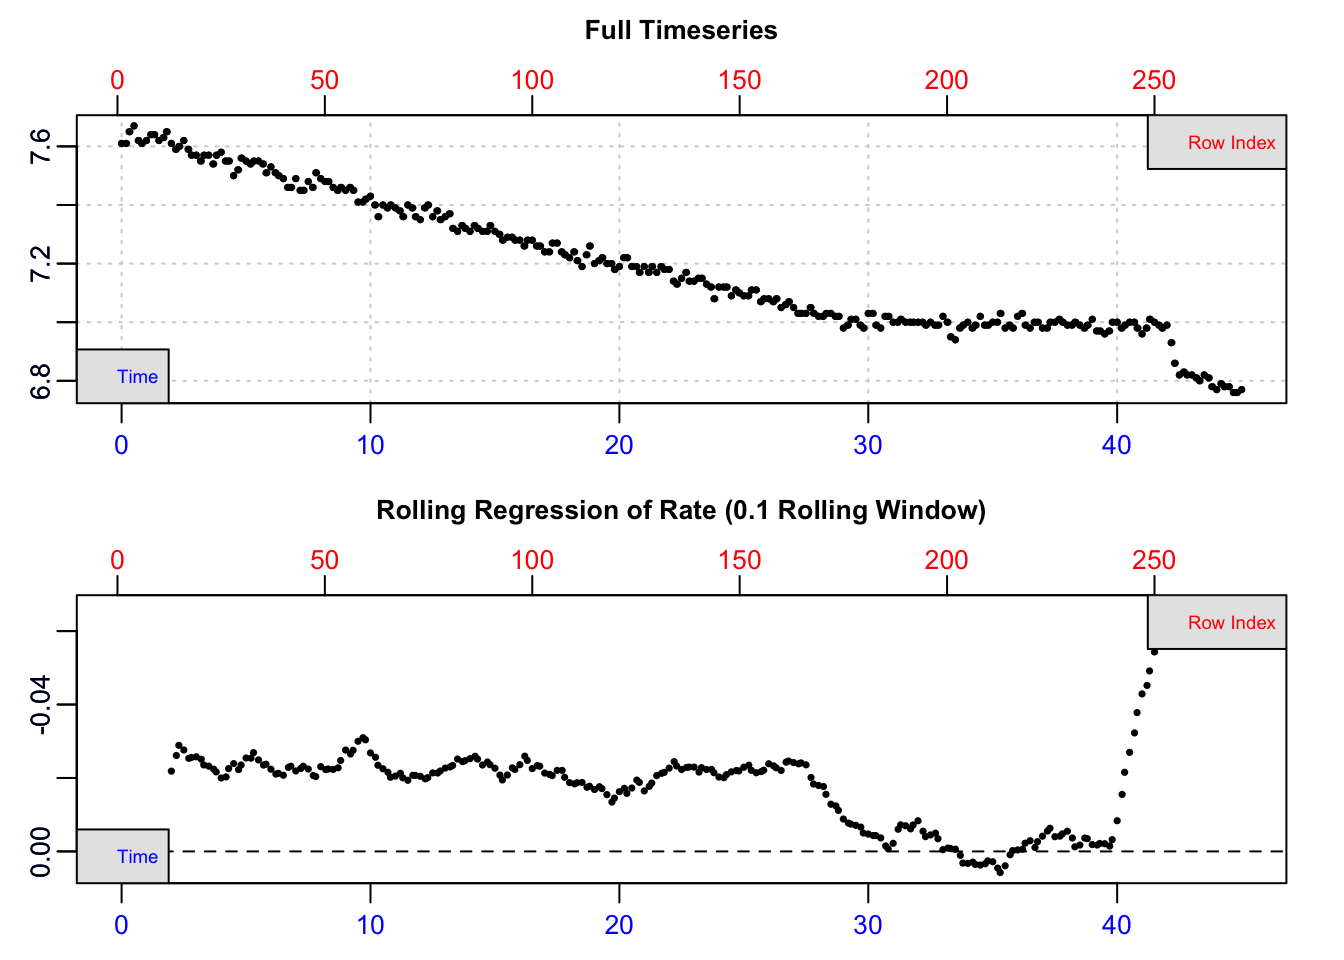
\includegraphics{respR_documentation_files/figure-latex/unnamed-chunk-16-1.pdf}

\begin{verbatim}
## 
## # inspect # -----------------------------
##               time.min    n
## NA/NAN            pass pass
## sequential        pass    -
## duplicated        pass    -
## evenly-spaced     WARN    -
## Uneven time data locations  (first 20 shown) in column: time.min n 
##  [1]  1  2  3  4  5  6  7  8  9 10 11 12 13 14 15 16 17 18 19 20
\end{verbatim}

\begin{verbatim}
## Warning: Time values are not evenly-spaced.
\end{verbatim}

From the plot, we can see irregularities in these data near the end of
the timeseries (in this case the specimen had interfered with the oxygen
sensor). A linear regression of the entire data series would therefore
give an erroneous calculation of the true rate. However, the bottom
output plot shows that over the initial stages of the experiment, oxygen
uptake shows a consistent rate, and so in this experiment this section
would be suitable for analysis.

The function also warns us that time data is not \emph{numerically}
evenly-spaced. However, \emph{this does not mean the data cannot be
processed}. Rather than make assumptions that rows represent evenly
spaced datapoints, the functions in \texttt{respR} use actual time
values for analyses and calculations, and so even irregularly spaced
data are analysed correctly. This warning is for information purposes
only: it is to make the user aware that if they use row numbers for
manual operations such as subsetting, the same width may not represent
the same time period. For now, the data frame is saved as an object,
\texttt{urchin} which contains the original data columns we selected
coerced into a data frame, and various other metadata.

\textbf{It should be noted that using \texttt{inspect()} is optional} -
the main functions in \texttt{respR} will readily accept regular
\texttt{R} data structures (e.g.~data frames, tibbles, vectors) as long
as data are numeric and error-free. Running \texttt{inspect()} is a
qualitative, exploratory step that highlights potential issues about the
data before analysis. We use this particular example, with an obvious
error towards the end, to illustrate the point that you should always
visualise and explore your data before analysis. \texttt{respR} has been
designed to make this easy.

\textbf{Note there is an older version of this function called
\texttt{inspect\_data()}} - this function has been deprecated, but kept
in the package to maintain compatibility with older code. It will not be
updated in the future, so users should use \texttt{inspect()}.

\section{Step 2: Process background
respiration}\label{step-2-process-background-respiration}

The presence of microorganisms may be a potential source of experimental
bias, and we may want to account for background respiration rates during
experiments. Since background rates typically account for a small
percentage of experimental rates, these often-called ``blank''
experiments are routinely conducted alongside, or before and after main
experiments, and often the rates are averaged across several datasets to
obtain a more accurate estimate of the correction.

The function \texttt{calc\_rate.bg()} can be used to simultaneously
process multiple background rate measurements as long as they share the
\textbf{same units of time and oxygen data as the experiments they will
be used to correct}. In \texttt{urchins.rd}, background respiration was
recorded and saved in columns 18 and 19. We analyse the data using the
specialised function \texttt{calc\_rate.bg()} and save the output as an
object. Note the function allows us to subset the data, here by
\texttt{time} from 5 to 40 minutes, to remove potentially erroneous
sections at the start (or end) before the system had reached stability.

\begin{Shaded}
\begin{Highlighting}[]
\CommentTok{# bg <- calc_rate.bg(urchins.rd, xcol = 1, ycol = 18:19, from = 5, to = 40, }
\CommentTok{#   by = "time")}
\CommentTok{# print(bg)}
\end{Highlighting}
\end{Shaded}

This object contains both individual background rates for each data
column entered, and an averaged rate which, by default, will be used as
the correction rate when this is applied later in \texttt{adjust\_rate}.

\section{Step 3: Calculate oxygen uptake
rate}\label{step-3-calculate-oxygen-uptake-rate}

Calling the function \texttt{calc\_rate()} on the \texttt{inspect()}
object, with no additional arguments, will prompt the function to
perform a linear regression on the entire data series.

\begin{Shaded}
\begin{Highlighting}[]
\KeywordTok{calc_rate}\NormalTok{(urchin) }\CommentTok{# same as: calc_rate(urchin$df)}
\end{Highlighting}
\end{Shaded}

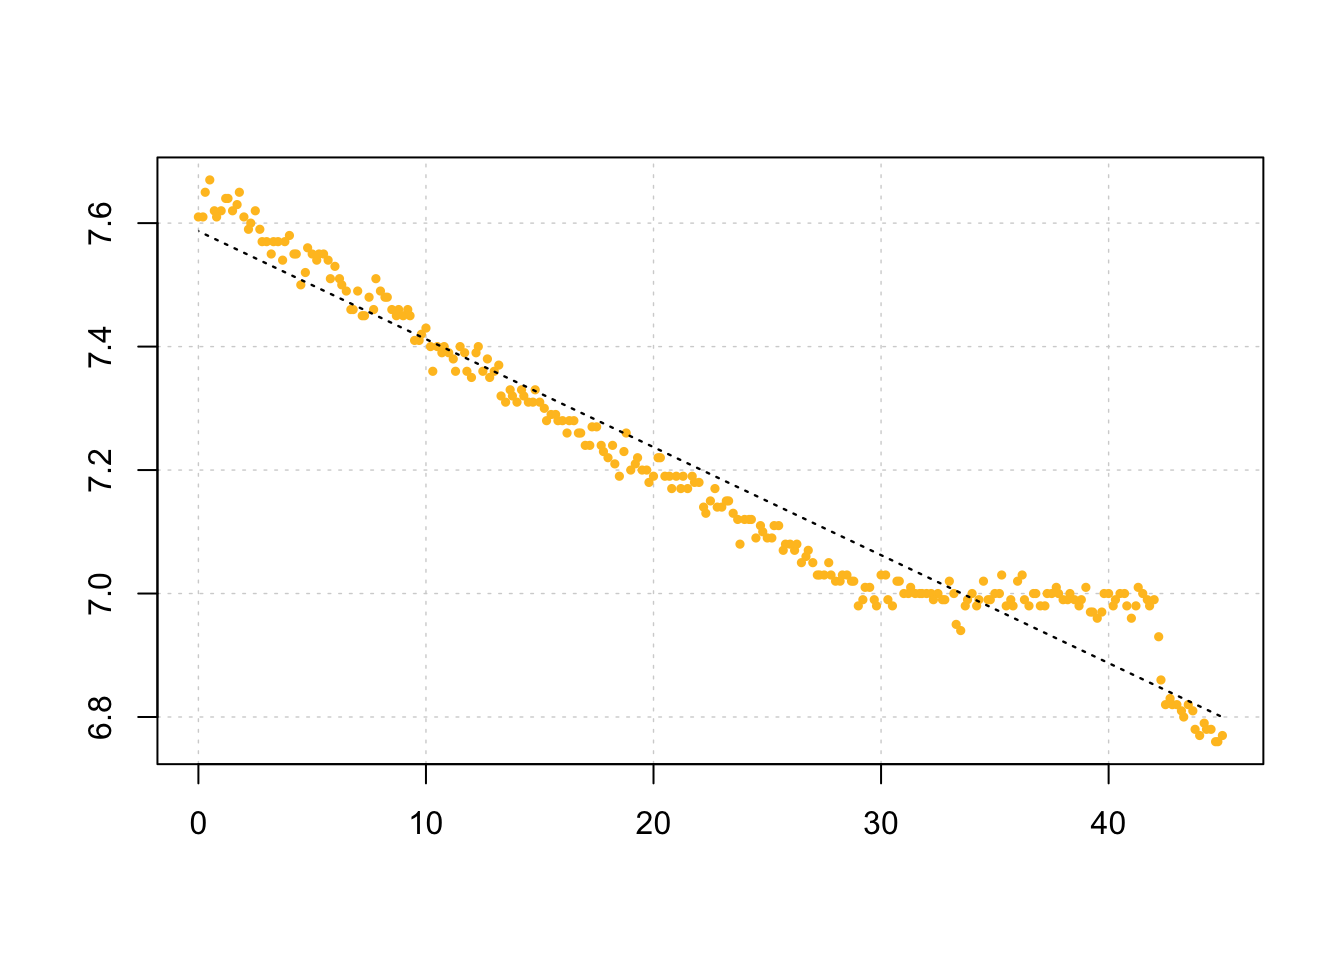
\includegraphics{respR_documentation_files/figure-latex/unnamed-chunk-19-1.pdf}

\begin{verbatim}
## 
## # calc_rate # -------------------
## Rate(s):
## [1] -0.01749242
\end{verbatim}

Note how the function recognises the \texttt{inspect()} object.
Alternatively, you can specify a \texttt{data.frame} object containing
raw data, in which case the function will automatically consider the
first column as time data, and the second column as dissolved \(O_2\)
data.

In many cases, there is a need to truncate or subset the data before
rate is determined. For example, we may want to determine rate over an
exact period of time, or within a threshold of O\textsubscript{2}
concentrations. Equipment interference or other factors may cause
irregularities in the data. We can work around such errors by subsetting
the regions that are not erroneous and still obtain valid results.

Based on the \texttt{from} and \texttt{to} arguments, a user may use
\texttt{calc\_rate()} to subset data in any of 4 ways:

\begin{enumerate}
\def\labelenumi{\arabic{enumi}.}
\tightlist
\item
  \textbf{Time period} (\texttt{by\ =\ "time"}) - \emph{``What is the
  rate over a specific 25 minute period?''}
\item
  \textbf{Total oxygen consumed} (\texttt{by\ =\ "o2"}) - \emph{``At
  what rate is oxygen consumed between saturation points of 95\% and
  80\%?''}
\item
  \textbf{Proportion based on total oxygen consumed}
  (\texttt{by\ =\ "proportion"}) - \emph{``What is the rate from 4/5ths
  (0.8) to halfway (0.5) along the data?''}
\item
  \textbf{Precise subsetting by row} (\texttt{by\ =\ "row"}). -
  \emph{``I'd like to determine rate between rows 11 and 273.''}
\end{enumerate}

We do not need to be overly precise; if input values of
O\textsubscript{2} and time do not match exactly to a value in the data,
the function will identify the closest matching values, rounded down,
and use these for subsequent calculations.

Here we'll select a 25 minute period before the interference occurred:

\begin{Shaded}
\begin{Highlighting}[]
\NormalTok{rate <-}\StringTok{ }\KeywordTok{calc_rate}\NormalTok{(urchin, }\DataTypeTok{from =} \DecValTok{4}\NormalTok{, }\DataTypeTok{to =} \DecValTok{29}\NormalTok{, }\DataTypeTok{by =} \StringTok{"time"}\NormalTok{)}
\end{Highlighting}
\end{Shaded}

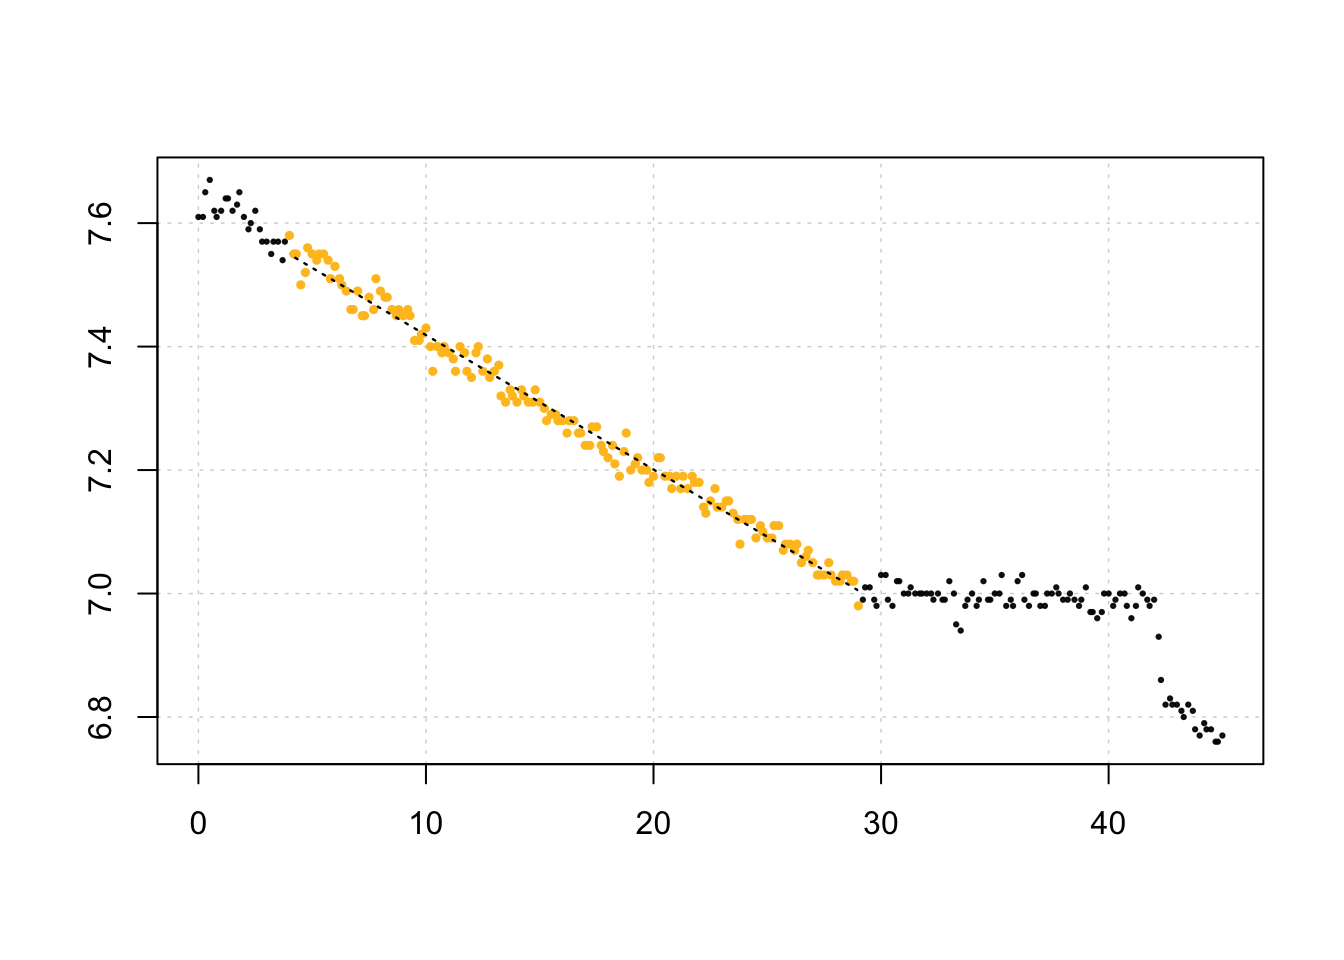
\includegraphics{respR_documentation_files/figure-latex/unnamed-chunk-20-1.pdf}

The saved object can be exported to a file, or explored using generic R
commands.

\begin{Shaded}
\begin{Highlighting}[]
\CommentTok{# uncomment to run and save as file}
\CommentTok{# write.csv(summary(rate), file = "results.csv")}

\KeywordTok{print}\NormalTok{(rate)}
\end{Highlighting}
\end{Shaded}

\begin{verbatim}
## 
## # calc_rate # -------------------
## Rate(s):
## [1] -0.02177588
\end{verbatim}

\begin{Shaded}
\begin{Highlighting}[]
\KeywordTok{summary}\NormalTok{(rate)}
\end{Highlighting}
\end{Shaded}

\begin{verbatim}
## Summary:
##    intercept_b0     rate_b1   rsq row endrow time endtime  oxy endoxy
## 1:     7.636454 -0.02177588 0.987  25    175    4      29 7.58   6.98
##    rowlength timelength rate_twopoint
## 1:       150         25        -0.024
\end{verbatim}

The rate can be seen as the second entry \texttt{rate\_b1}, and other
summary data are saved in the object. The output also includes a
\texttt{rate\_2pt}. This is the rate determined by simple two-point
calculation of difference in O\textsubscript{2} divided by difference in
Time. For almost all analyses, the \texttt{rate\_b1} should be used. See
\href{https://januarharianto.github.io/respR/articles/twopoint.html}{Two-point
analyses} for an explanation of this output and when it should be used.

Plotting the output provides a series of diagnostic plots of the data
subset that was analysed.

\begin{Shaded}
\begin{Highlighting}[]
\KeywordTok{plot}\NormalTok{(rate)}
\end{Highlighting}
\end{Shaded}

\begin{verbatim}
## 
## # plot # ------------------------
## Plotting...this may take a while for large datasets.
\end{verbatim}

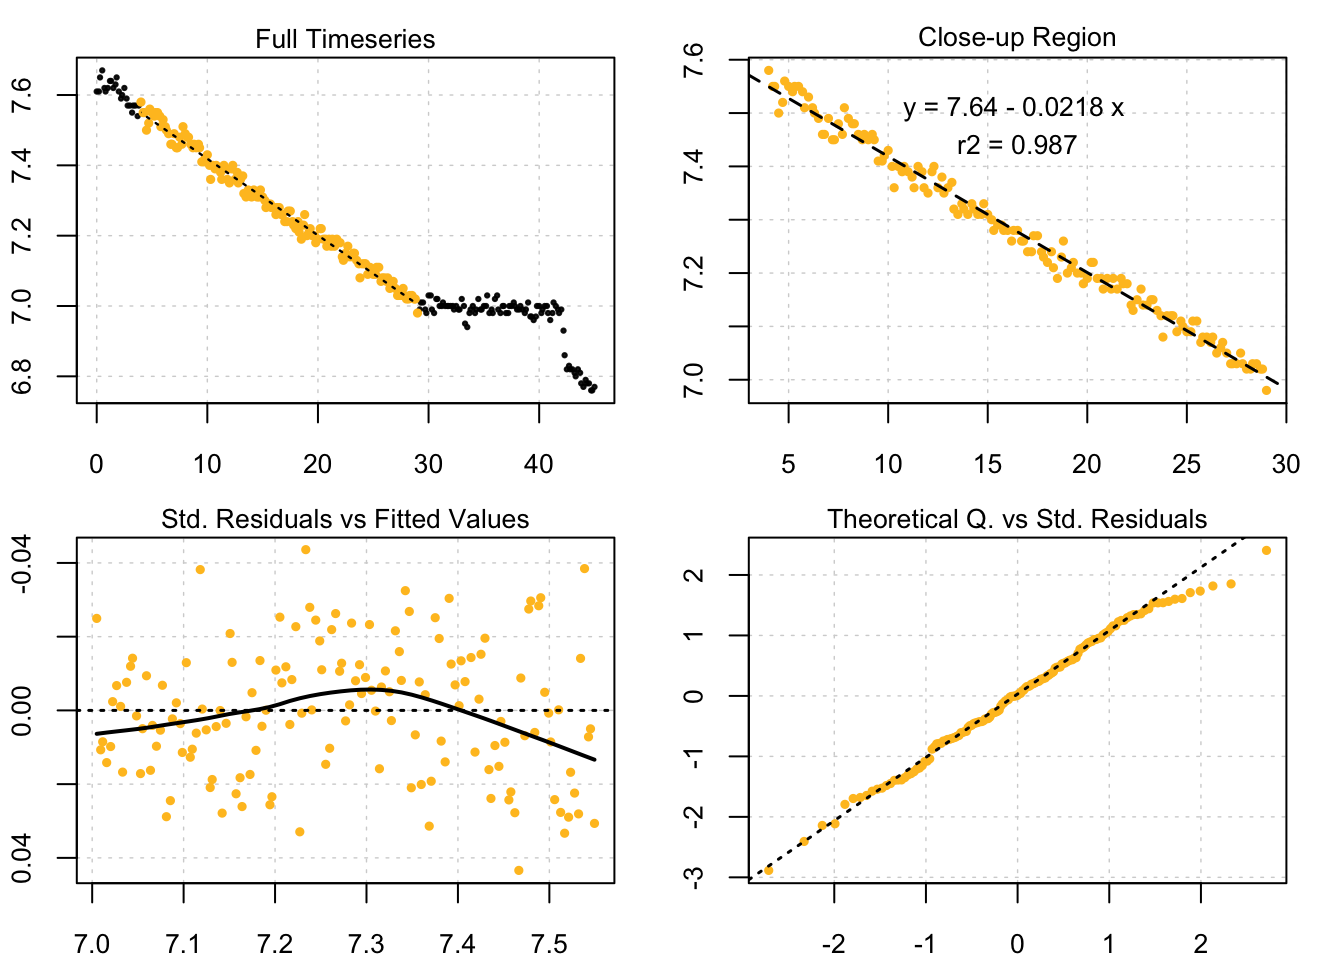
\includegraphics{respR_documentation_files/figure-latex/unnamed-chunk-22-1.pdf}

\begin{verbatim}
## Done.
\end{verbatim}

\section{Step 4: Adjust for background
respiration}\label{step-4-adjust-for-background-respiration}

Since background rate has been calculated in \texttt{calc\_rate.bg()},
adjustment is straightforward using the function
\texttt{adjust\_rate()}. The \texttt{rate} input can be an object of
class \texttt{calc\_rate} or \texttt{auto\_rate}, or any numeric value.

\begin{Shaded}
\begin{Highlighting}[]
\CommentTok{# a.rate <- adjust_rate(rate, bg)}
\CommentTok{# a.rate}
\end{Highlighting}
\end{Shaded}

A background correction can also be entered manually. Care should be
taken to include the correct (typically negative) sign.

\begin{Shaded}
\begin{Highlighting}[]
\NormalTok{a.rate <-}\StringTok{ }\KeywordTok{adjust_rate}\NormalTok{(rate, }\OperatorTok{-}\FloatTok{0.00083}\NormalTok{)}
\end{Highlighting}
\end{Shaded}

\begin{verbatim}
## 
## Rate adjustments applied. Use print() command for more info.
\end{verbatim}

\begin{Shaded}
\begin{Highlighting}[]
\NormalTok{a.rate}
\end{Highlighting}
\end{Shaded}

\begin{verbatim}
## 
## # adjust_rate # -------------------------
## Note: please consider the sign of the value while correcting the rate.
## 
## Rank/position 1 result shown. To see all results use summary().
## Input rate: -0.02177588
## Adjustment: -0.00083
## Adj. rate: -0.02094588
\end{verbatim}

For experiments where there is a quantified background \textbf{input} of
oxygen, such as in \emph{open-tank} respirometry,
\texttt{adjust\_rate()} can be used to correct rates using a
\emph{positive} background value.

\begin{Shaded}
\begin{Highlighting}[]
\NormalTok{a.rate <-}\StringTok{ }\KeywordTok{adjust_rate}\NormalTok{(rate, }\FloatTok{0.002}\NormalTok{)}
\end{Highlighting}
\end{Shaded}

\begin{verbatim}
## 
## Rate adjustments applied. Use print() command for more info.
\end{verbatim}

\begin{Shaded}
\begin{Highlighting}[]
\NormalTok{a.rate}
\end{Highlighting}
\end{Shaded}

\begin{verbatim}
## 
## # adjust_rate # -------------------------
## Note: please consider the sign of the value while correcting the rate.
## 
## Rank/position 1 result shown. To see all results use summary().
## Input rate: -0.02177588
## Adjustment: 0.002
## Adj. rate: -0.02377588
\end{verbatim}

\section{Step 5: Convert the results}\label{step-5-convert-the-results}

Note, that until this point \texttt{respR} has \textbf{not required
units of time or oxygen to be entered}. Here, we convert calculated,
unitless rates to specified output units.

For example, we may want to calculate:

\begin{enumerate}
\def\labelenumi{\arabic{enumi}.}
\tightlist
\item
  \(\dot{V}O_2\) - Total change in O\textsubscript{2} per unit time
  within the chamber; or
\item
  \(\dot{M}O_2\) - Mass-specific rate of change in O\textsubscript{2}
  per unit time of the specimen.
\end{enumerate}

The function \texttt{convert\_rate()} can be used to convert rate values
to chamber volume and/or specimen mass specific values. This requires
the units of the original data (\texttt{o2.unit}, \texttt{time.unit}),
and in SI units (L, kg) the \texttt{volume} of fluid in the chamber, and
\texttt{mass} of the specimen.

\textbf{Note:} the \texttt{volume} is volume of water in the
respirometer, \textbf{not the volume of the respirometer}. That is, it
represents the effective volume; a specimen might displace a significant
proportion of the water, depending on its size. Therefore the volume of
water entered here should equal the volume of the respirometer
\textbf{minus the volume of the specimen}. It depends on your experiment
how you determine water volume. There are several approaches to
calculate the volume of a specimen; geometrically, through displacement
in a separate vessel, or calculated from the mass assuming a density
value (e.g.~for fish it is often assumed they have an equal density as
water, that is \textasciitilde{}1000 kg/m\^{}3). Volume could also be
determined directly by pouring out the water at the end of the
experiment, or by a weighing approach.

For an example of \(VO_2\), or absolute oxygen uptake rate, we may
convert the output of \texttt{calc\_rate()} to O\textsubscript{2}
consumed per hour:

\begin{Shaded}
\begin{Highlighting}[]
\KeywordTok{convert_rate}\NormalTok{(a.rate, }
             \DataTypeTok{o2.unit =} \StringTok{"mg/L"}\NormalTok{, }
             \DataTypeTok{time.unit =} \StringTok{"min"}\NormalTok{, }
             \DataTypeTok{output.unit =} \StringTok{"mg/h"}\NormalTok{, }
             \DataTypeTok{volume =} \FloatTok{1.09}\NormalTok{)}
\end{Highlighting}
\end{Shaded}

\begin{verbatim}
## 
## # convert_rate # ------------------------
## Rank/position 1 result shown. To see all results use summary().
## Input:
## [1] -0.02377588
## [1] "mg/L" "min" 
## Converted:
## [1] -1.554943
## [1] "mg/hour"
\end{verbatim}

We can also convert the rate to a volume-corrected, mass-specific rate:

\begin{Shaded}
\begin{Highlighting}[]
\KeywordTok{convert_rate}\NormalTok{(a.rate, }
             \DataTypeTok{o2.unit =} \StringTok{"mgl-1"}\NormalTok{, }
             \DataTypeTok{time.unit =} \StringTok{"m"}\NormalTok{, }
             \DataTypeTok{output.unit =} \StringTok{"mg/s/kg"}\NormalTok{,}
             \DataTypeTok{volume =} \FloatTok{1.09}\NormalTok{, }
             \DataTypeTok{mass =} \FloatTok{0.19}\NormalTok{)}
\end{Highlighting}
\end{Shaded}

\begin{verbatim}
## 
## # convert_rate # ------------------------
## Rank/position 1 result shown. To see all results use summary().
## Input:
## [1] -0.02377588
## [1] "mg/L" "min" 
## Converted:
## [1] -0.002273308
## [1] "mg/sec/kg"
\end{verbatim}

A ``fuzzy'' string matching algorithm is used to automatically recognise
variations in base units, allowing natural, intuitive input of units.
For example, \texttt{"ml/s"}, \texttt{"mL/sec"},
\texttt{"milliliter/s"}, and \texttt{"millilitre/second"} are all
equally identified as \texttt{mL/s}. Unit delimiters can be any
combination of a space, dot (\texttt{.}), forward-slash (\texttt{/}), or
the ``per'' unit (\texttt{-1}). Thus, \texttt{"ml/kg"},
\texttt{"mL\ /\ kg"}, \texttt{"mL\ /kilogram"}, \texttt{"ml\ kg-1"} or
\texttt{"ml.kg-1"} are equally recognised as \texttt{mL/kg}. For a
reminder on what units are available to use, call \texttt{unit\_args()}:

\begin{Shaded}
\begin{Highlighting}[]
\KeywordTok{unit_args}\NormalTok{()}
\end{Highlighting}
\end{Shaded}

\begin{verbatim}
## Note: A string-matching algorithm is used to identify units. 
## E.g. all of these are the same: mg/L; mg/l, mg L-1, mgL-1, mg per litre, mg.l-1, mg.L-1
## 
## O2 Units - Do not require t, S and P
## [1] "mg/L"   "ug/L"   "mmol/L" "umol/L"
## 
## O2 Units - Require t, S and P
##  [1] "mL/L"    "mg/kg"   "ug/kg"   "mmol/kg" "umol/kg" "mL/kg"   "%"      
##  [8] "Torr"    "hPa"     "kPa"     "mmHg"    "inHg"   
## 
## Time units
## [1] "s" "m" "h"
## 
## Output mass units
## [1] "ug" "mg" "g"  "kg"
\end{verbatim}

\section{Summary}\label{summary}

This is an example of a straightforward analysis of a
\emph{closed-chamber} respirometry experiment. This entire analysis can
be documented and shared in only a few lines of code, making it entirely
reproducible if the original data file is included:

\begin{Shaded}
\begin{Highlighting}[]
\CommentTok{# # import and inspect}
\CommentTok{# urchin <- inspect(urchins.rd, time = 1, oxygen = 15)}
\CommentTok{# }
\CommentTok{# # Background}
\CommentTok{# bg <- calc_rate.bg(urchins.rd, xcol = 1, ycol = 18:19, from = 5, to = 40, by = "time")}
\CommentTok{# }
\CommentTok{# # Specimen rate}
\CommentTok{# rate <- calc_rate(urchin, from = 4, to = 29, by = "time")}
\CommentTok{# }
\CommentTok{# # Adjust rate}
\CommentTok{# a.rate <- adjust_rate(rate, bg)}
\CommentTok{# }
\CommentTok{# # Convert to final rate units}
\CommentTok{# urchin_MO2 <- convert_rate(a.rate,}
\CommentTok{#                            o2.unit = "mgl-1", }
\CommentTok{#                            time.unit = "m", }
\CommentTok{#                            output.unit = "mg/s/kg", }
\CommentTok{#                            volume = 1.09, }
\CommentTok{#                            mass = 0.19)}
\CommentTok{# }
\CommentTok{# # Alternatively, use dplyr pipes, adding a print() between functions:}
\CommentTok{# }
\CommentTok{# urchins.rd %>%                                           # With the data object,}
\CommentTok{#   inspect(1, 15) %>%                                     # inspect, then}
\CommentTok{#   calc_rate(from = 4, to = 29, by = "time") %>%          # calculate rate, then}
\CommentTok{#   print() %>%}
\CommentTok{#   adjust_rate(}
\CommentTok{#     calc_rate.bg(urchins.rd, xcol = 1, ycol = 18:19,     # adjust bg rate, then}
\CommentTok{#       from = 5, to = 40, by = "time")) %>%}
\CommentTok{#   print() %>%}
\CommentTok{#   convert_rate(o2.unit = "mgl-1", time.unit = "m",     }
\CommentTok{#     output.unit = "mg/s/kg", volume = 1.09, mass = 0.19) # convert units.}
\end{Highlighting}
\end{Shaded}

\chapter{\texorpdfstring{Using
\texttt{auto\_rate()}}{Using auto\_rate()}}\label{using-auto_rate}

--\textgreater{} --\textgreater{} --\textgreater{} --\textgreater{}

--\textgreater{}

--\textgreater{}

--\textgreater{} --\textgreater{} --\textgreater{} --\textgreater{}

--\textgreater{}

--\textgreater{}

--\textgreater{} --\textgreater{} --\textgreater{}

\chapter{Performance in detecting linear
regions}\label{performance-in-detecting-linear-regions}

\chapter{\texorpdfstring{Comparative performance of
\texttt{auto\_rate()} and
\texttt{LoLinR}}{Comparative performance of auto\_rate() and LoLinR}}\label{comparative-performance-of-auto_rate-and-lolinr}

--\textgreater{}

--\textgreater{}

--\textgreater{} --\textgreater{}

--\textgreater{}

--\textgreater{}

--\textgreater{} --\textgreater{}

\chapter{Intermittent-flow respirometry: Simple
example}\label{intermittent-flow-respirometry-simple-example}

\chapter{Intermittent-flow respirometry: Complex
example}\label{intermittent-flow-respirometry-complex-example}

\chapter{Flowthrough respirometry}\label{flowthrough-respirometry}

\chapter{\texorpdfstring{P\textsubscript{crit}}{Pcrit}}\label{pcrit}

\chapter{Two-point analyses}\label{two-point-analyses}

\chapter{Open science and reproducibility using
respR}\label{open-science-and-reproducibility-using-respr}

\chapter{respR and the tidyverse}\label{respr-and-the-tidyverse}

\section{Working in the Tidyverse}\label{working-in-the-tidyverse}

\chapter{A comparison of respR with other R
packages}\label{a-comparison-of-respr-with-other-r-packages}

\chapter{When to use respR}\label{when-to-use-respr}

--\textgreater{} --\textgreater{}

--\textgreater{} --\textgreater{} --\textgreater{}

--\textgreater{}

--\textgreater{}

\bibliography{book.bib,packages.bib}


\end{document}
